\hspace{\parindent}  Two main types of testing have been done for this version of the app - Unit testing and Firebase testing. Unit testing could not have been done through the usual means as JUnit tests, but rather as ordinary tests due asynchronous nature of Firebase, which makes it impossible to test with JUnit tests. \newline

The only real JUnit test is done for AES encryption/decryption. More on that can be found in the latter subsections. \newline




\subsection{Unit testing}
\hspace{\parindent} 
Unit testing has been done for the following actions of fetching Firebase data:
\begin{itemize}
\item \textbf{Fetching store cities}
\begin{figure}[H]
\centering
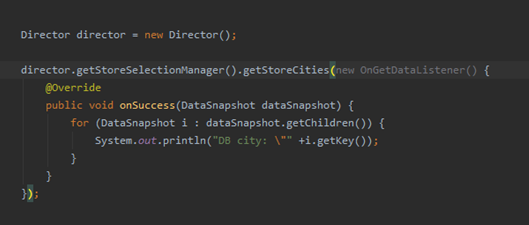
\includegraphics[width=0.9\textwidth]{Images/TestingPics/StoreCities1}
\caption{\label{fig:test1}\textbf{Fetching store cities test 1}}
\end{figure}
\begin{figure}[H]
\centering
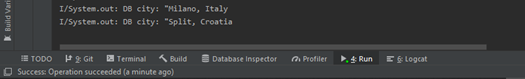
\includegraphics[width=0.9\textwidth]{Images/TestingPics/StoreCities2}
\caption{\label{fig:test2}\textbf{Fetching store cities test 2}}
\end{figure}
\item \textbf{Fetching store chains in a city}
\begin{figure}[H]
\centering
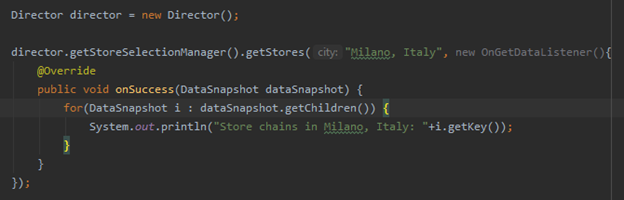
\includegraphics[width=0.9\textwidth]{Images/TestingPics/StoreChains1}
\caption{\label{fig:test3}\textbf{Fetching store chains in a city test 1}}
\end{figure}
\begin{figure}[H]
\centering
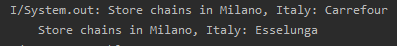
\includegraphics[width=0.9\textwidth]{Images/TestingPics/StoreChains2}
\caption{\label{fig:test4}\textbf{Fetching store chains in a city test 2}}
\end{figure}
\item \textbf{Fetching store chain addresses}
\begin{figure}[H]
\centering
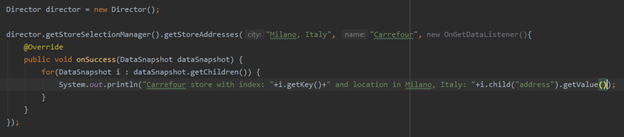
\includegraphics[width=0.9\textwidth]{Images/TestingPics/StoreChainAddresses1}
\caption{\label{fig:test5}\textbf{Fetching store chain addresses test 1}}
\end{figure}
\begin{figure}[H]
\centering
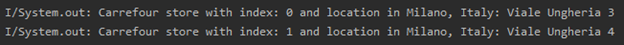
\includegraphics[width=0.9\textwidth]{Images/TestingPics/StoreChainAddresses2}
\caption{\label{fig:test6}\textbf{Fetching store chain addresses test 2}}
\end{figure}
\item \textbf{Checking credentials for a store manager login}
\begin{figure}[H]
\centering
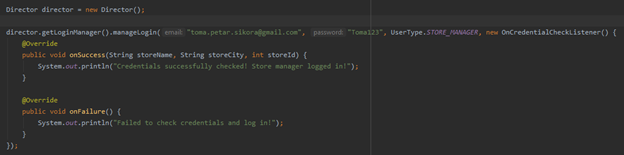
\includegraphics[width=0.9\textwidth]{Images/TestingPics/LoginOK1}
\caption{\label{fig:test7}\textbf{Successful login test}}
\end{figure}
\begin{figure}[H]
\centering
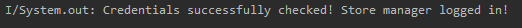
\includegraphics[width=0.9\textwidth]{Images/TestingPics/LoginOK2}
\caption{\label{fig:test8}\textbf{Successful login test results}}
\end{figure}
\begin{figure}[H]
\centering
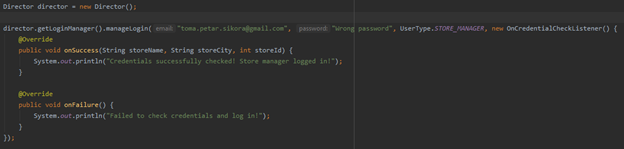
\includegraphics[width=0.9\textwidth]{Images/TestingPics/LoginBad1}
\caption{\label{fig:test9}\textbf{Failed login test}}
\end{figure}
\begin{figure}[H]
\centering
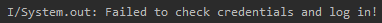
\includegraphics[width=0.9\textwidth]{Images/TestingPics/LoginBad2}
\caption{\label{fig:test10}\textbf{Failed login test results}}
\end{figure}
\item \textbf{Acquiring ticket to get in the virtual line}
\begin{figure}[H]
\centering
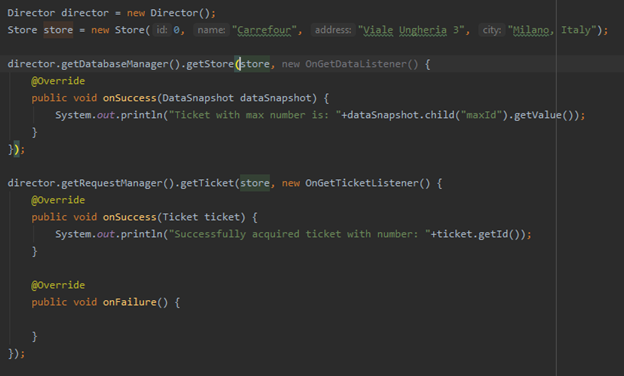
\includegraphics[width=0.9\textwidth]{Images/TestingPics/GetTicket1}
\caption{\label{fig:test11}\textbf{Acquiring ticket test}}
\end{figure}
\begin{figure}[H]
\centering
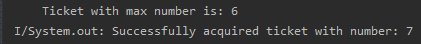
\includegraphics[width=0.9\textwidth]{Images/TestingPics/GetTicket2}
\caption{\label{fig:test12}\textbf{Acquiring ticket test results}}
\end{figure}
\item \textbf{Checking the state of the ticket}
\begin{figure}[H]
\centering
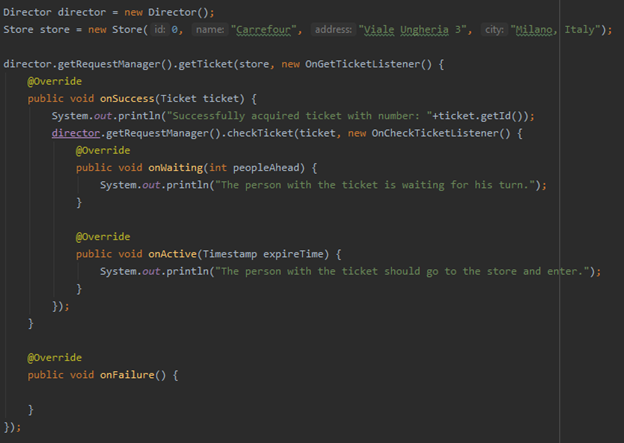
\includegraphics[width=0.9\textwidth]{Images/TestingPics/TicketState1}
\caption{\label{fig:test13}\textbf{Checking the state of the ticket test }}
\end{figure}
\begin{figure}[H]
\centering
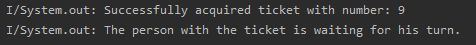
\includegraphics[width=0.9\textwidth]{Images/TestingPics/TicketState2}
\caption{\label{fig:test14}\textbf{Checking the state of the ticket test results}}
\end{figure}
\item \textbf{Cancelling the ticket}
\begin{figure}[H]
\centering
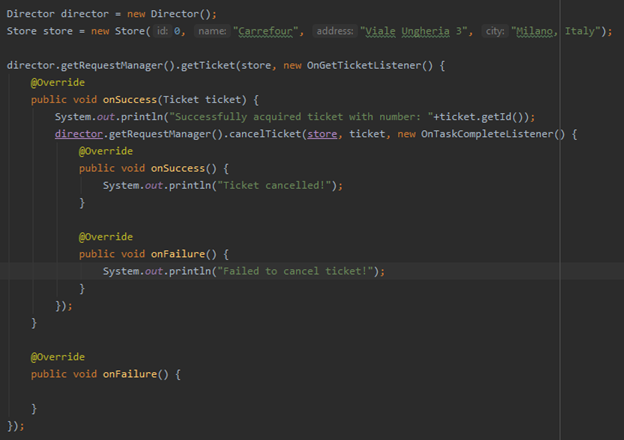
\includegraphics[width=0.9\textwidth]{Images/TestingPics/CancelTicket1}
\caption{\label{fig:test15}\textbf{Cancelling the ticket test}}
\end{figure}
\begin{figure}[H]
\centering
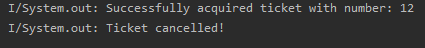
\includegraphics[width=0.9\textwidth]{Images/TestingPics/CancelTicket2}
\caption{\label{fig:test16}\textbf{Cancelling the ticket test results}}
\end{figure}
\item \textbf{Checking ticket logic 1}

Beginning state:\newline
Maximum store occupancy is 2, current occupancy is 0.
There are 2 active tickets with numbers 11 and 12, with expire time 11:01 ( 5 minutes after activation), 3 waiting tickets with numbers 13, 14, and 15.\newline

\begin{figure}[H]
\centering
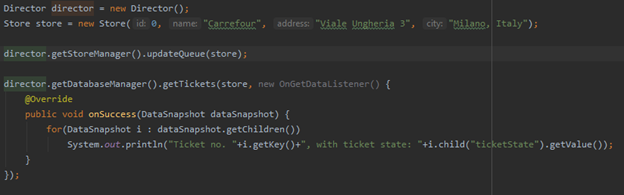
\includegraphics[width=0.9\textwidth]{Images/TestingPics/Test11}
\caption{\label{fig:test17}\textbf{Checking ticket logic test 1.1}}
\end{figure}
\begin{figure}[H]
\centering
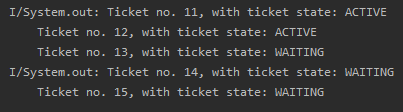
\includegraphics[width=0.9\textwidth]{Images/TestingPics/Test12}
\caption{\label{fig:test18}\textbf{Checking ticket logic test 1.1 results}}
\end{figure}

Customer with ticket number 11 scans his ticket and the store manager lets him in.

\begin{figure}[H]
\centering
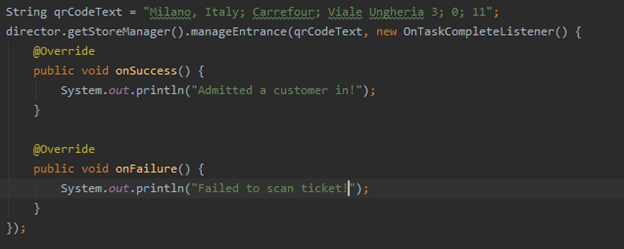
\includegraphics[width=0.9\textwidth]{Images/TestingPics/Test13}
\caption{\label{fig:test19}\textbf{Checking ticket logic test 1.2}}
\end{figure}
\begin{figure}[H]
\centering
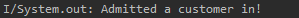
\includegraphics[width=0.9\textwidth]{Images/TestingPics/Test14}
\caption{\label{fig:test20}\textbf{Checking ticket logic test 1.2 results}}
\end{figure}
After a couple of minutes, store manager automatically updates the queue:\newline
In the meantime, ticket with number 12 has expired, and the ticket with number 13 is activated.

\begin{figure}[H]
\centering
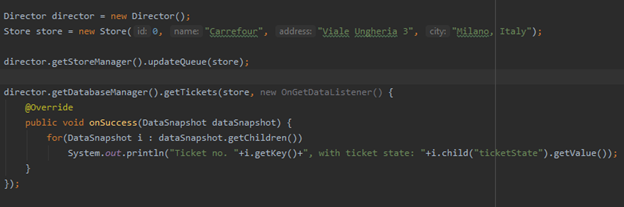
\includegraphics[width=0.9\textwidth]{Images/TestingPics/Test15}
\caption{\label{fig:test21}\textbf{Checking ticket logic test 1.3}}
\end{figure}
\begin{figure}[H]
\centering
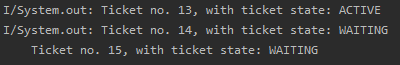
\includegraphics[width=0.9\textwidth]{Images/TestingPics/Test16}
\caption{\label{fig:test22}\textbf{Checking ticket logic test 1.3 results}}
\end{figure}

When a customer exits, the occupancy changes and another customers ticket is activated.

\begin{figure}[H]
\centering
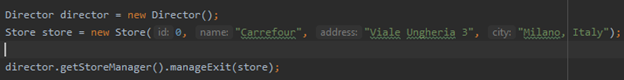
\includegraphics[width=0.9\textwidth]{Images/TestingPics/Test17}
\caption{\label{fig:test23}\textbf{Checking ticket logic test 1.4}}
\end{figure}
\begin{figure}[H]
\centering
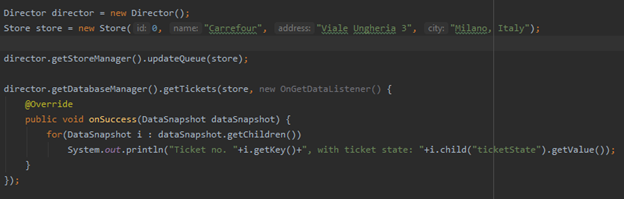
\includegraphics[width=0.9\textwidth]{Images/TestingPics/Test18}
\caption{\label{fig:test24}\textbf{Checking ticket logic test 1.5}}
\end{figure}
\begin{figure}[H]
\centering
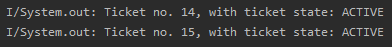
\includegraphics[width=0.9\textwidth]{Images/TestingPics/Test19}
\caption{\label{fig:test25}\textbf{Checking ticket logic test 1.4 and 1.5 results}}
\end{figure}


\item \textbf{Checking ticket logic 2}

Beginning state:\newline
Maximum store occupancy is 2, tickets with number 1 and 2 are activated, ticket with number 3 is waiting.
Person with ticket number 3 tries to enter the store before his ticket is activated.\newline

\begin{figure}[H]
\centering
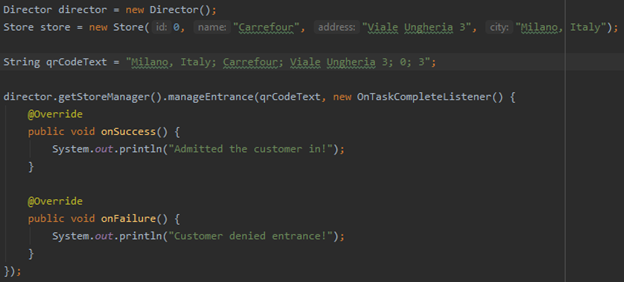
\includegraphics[width=0.9\textwidth]{Images/TestingPics/Test21}
\caption{\label{fig:test25}\textbf{Checking ticket logic test 2}}
\end{figure}
\begin{figure}[H]
\centering
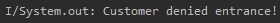
\includegraphics[width=0.9\textwidth]{Images/TestingPics/Test22}
\caption{\label{fig:test26}\textbf{Checking ticket logic test 2 results}}
\end{figure}

\end{itemize}


\newpage
\subsection{Firebase testing} 
\hspace{\parindent} Firebase has its own implemented testing that tests the stress the app puts on the system. It crawls through the entire app and returns results based on memory, network, and CPU usage. It also takes into account UI responsiveness and framerate.\newline

Here are the results of Firebase testing:\newline 

\begin{figure}[H]
\centering
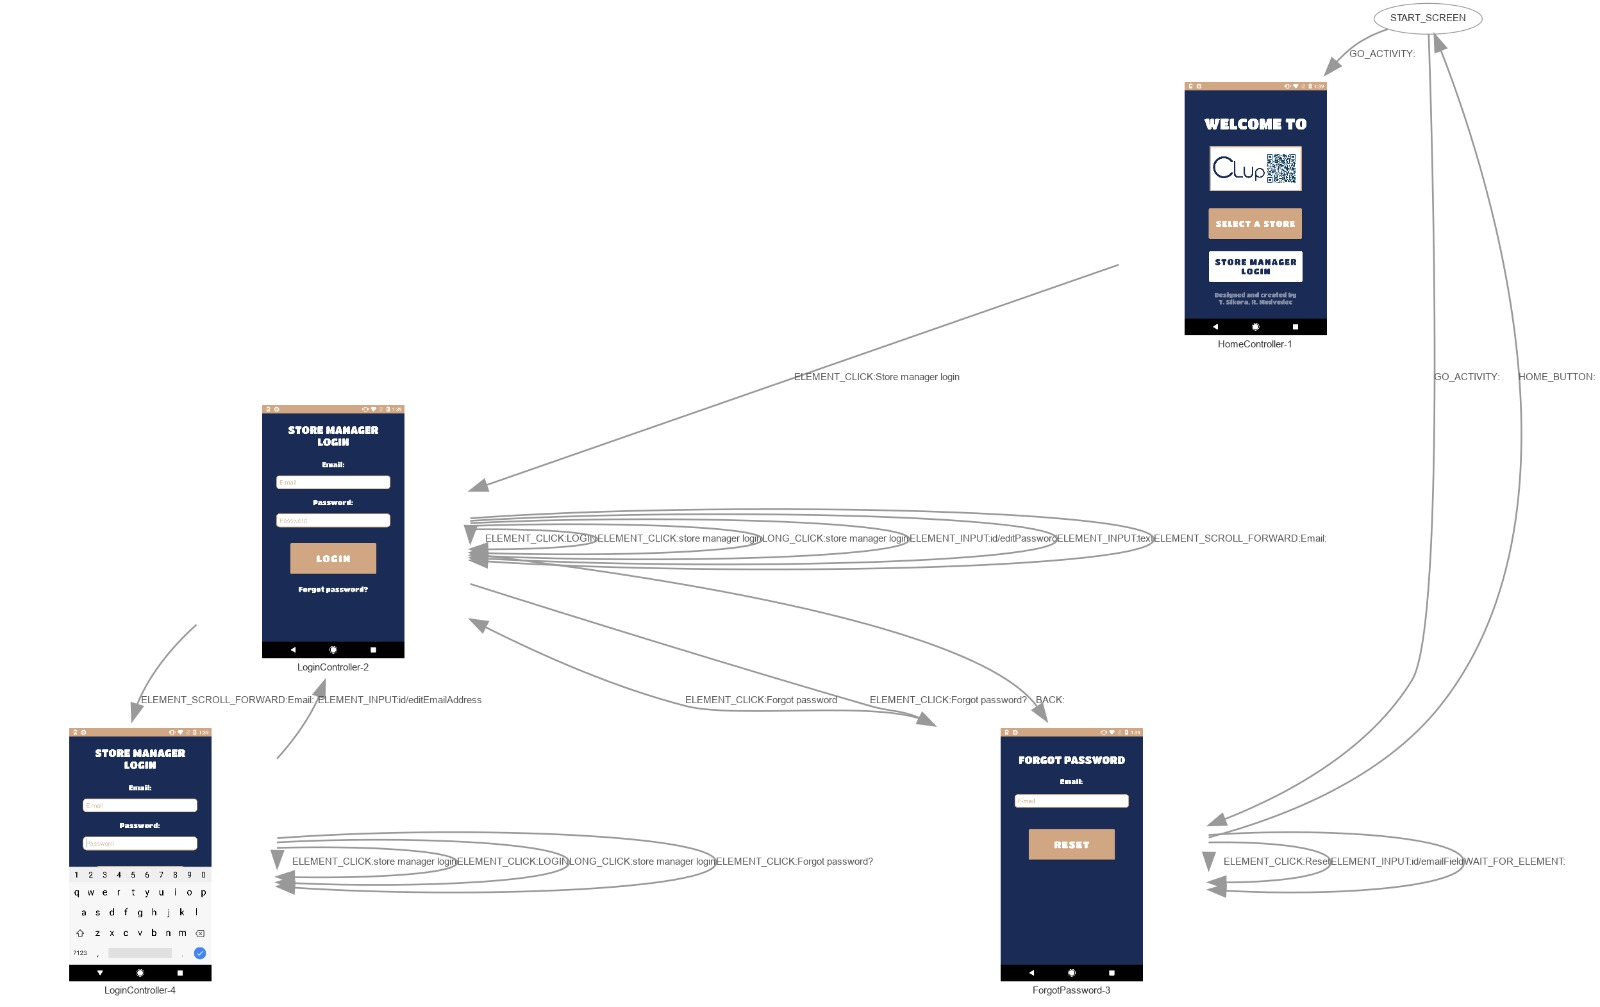
\includegraphics[width=\textwidth]{Images/TestingPics/Test1}
\caption{\label{fig:test26}\textbf{Firebase test crawling diagram}}
\end{figure}
\begin{figure}[H]
\centering
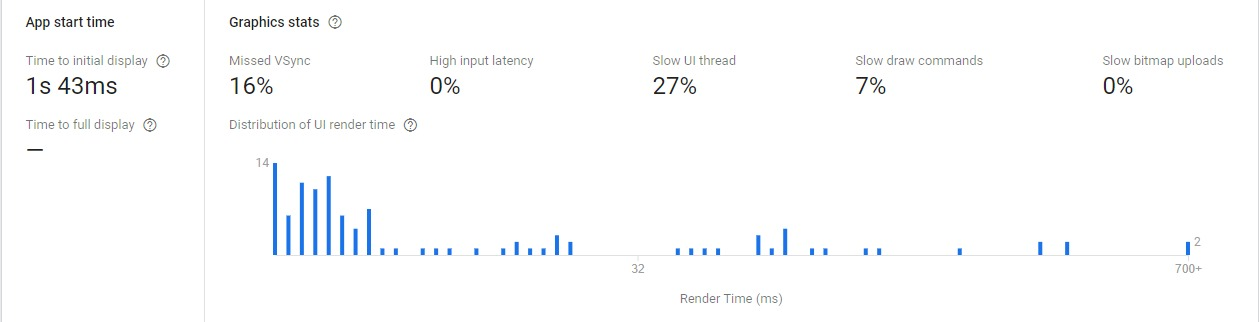
\includegraphics[width=\textwidth]{Images/TestingPics/Test2}
\caption{\label{fig:test27}\textbf{Firebase test UI responsiveness}}
\end{figure}
\begin{figure}[H]
\centering
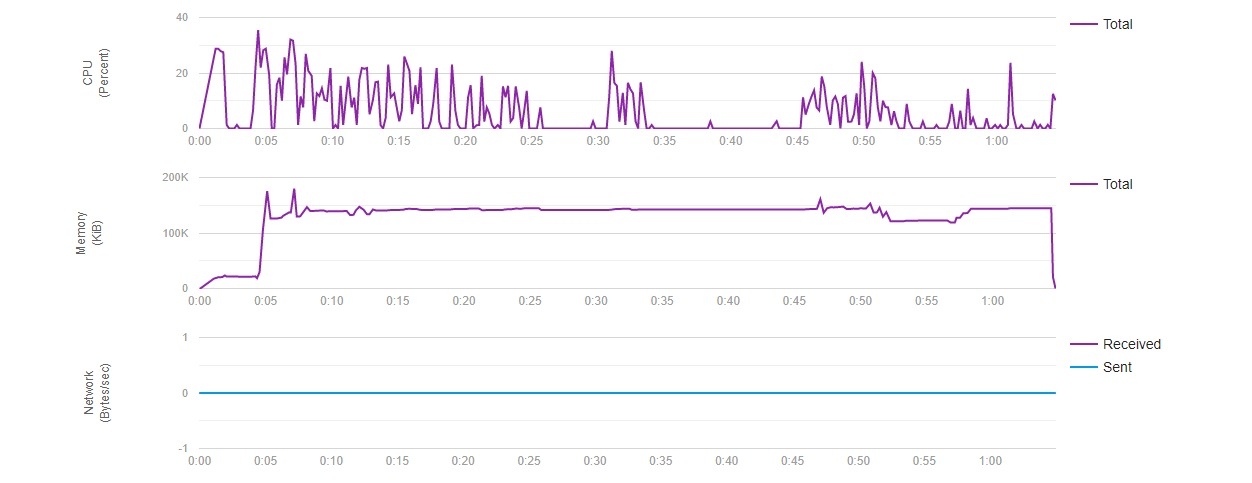
\includegraphics[width=\textwidth]{Images/TestingPics/Test3}
\caption{\label{fig:test28}\textbf{Firebase test performance and resource usage}}
\end{figure}

\subsection{Security testing}
\hspace{\parindent} The only real JUnit test from Android Studio was ran on this component and the code looks like this:

\begin{lstlisting}
// Hello.java
package com.example.clup;

import org.junit.Test;

import static org.junit.Assert.assertEquals;


/**
 * Local unit test to test whether AES encryption of tickets works as intended.
 * The test will execute on the development machine (host).
 */
public class EncryptionUnitTest {
    @Test
    public void encryption_is_correct() {
        StrongAES strongAES = new StrongAES();
        String text = "This text should remain the same after encryption and decryption.";
        String key = "YaBcmo5Tz3hb8piW";
        assertEquals(text, strongAES.AESDecrypt(strongAES.AESEncrypt(text, key), key));
    }
}

\end{lstlisting}

The code returns the correct value which means that the test is passed.

